\documentclass[twoside]{homework}

\usepackage{dsfont} 

\usepackage{graphicx}
\usepackage{listings}
\usepackage{amsmath}
\usepackage{bm}
\usepackage{xcolor}
\lstset{
    rulesepcolor= \color{gray}, %代码块边框颜色
    breaklines=true,  %代码过长则换行
    numbers=left, %行号在左侧显示
    numberstyle= \small,%行号字体
    %keywordstyle= \color{red},%关键字颜色
    commentstyle=\color{gray}, %注释颜色
    frame=shadowbox%用方框框住代码块
}

\studname{Chenye Yang}
\uni{cy2540}
\studmail{cy2540@columbia.edu}
\coursename{Statistical Learning for Biological and Information Systems}
\hwNo{1}

\begin{document}
\maketitle

\section*{P1}

\subsection*{(a)}
\textbf{Ans:}\\
\begin{equation}
\begin{aligned}
(n-1)S^2+n\bar{X}^2 &= \sum_{i=1}^{n} (X_i-\bar{X})^2 + n\bar{X}^2\\
&= \sum_{i=1}^{n}X_i^2 - 2\bar{X} \sum_{i=1}^{n} X_i +2n\bar{X}^2\\
&= \sum_{i=1}^{n}X_i^2 - 2\bar{X} n \bar{X} +2n\bar{X}^2\\
&= \sum_{i=1}^{n}X_i^2
\end{aligned}
\end{equation}

\subsection*{(b)}
\textbf{Ans:}\\
Because $X_1, X_2, ..., X_n$ are independent and identically distributed, using $a$ as the expected value of the distribution, we have $\mathbb{E}(X_i)=\mathbb{E}(\bar{X})=a$. \\
Thus: 
\begin{equation}
\begin{aligned}
    \sum_{i=1}^n (X_i - \bar{X})^2 &= \sum_{i=1}^n [(X_i - a)-(\bar{X}-a)]^2 \\
    &=  \sum_{i=1}^n [(X_i - a)^2 -2(X_i - a)(\bar{X}-a) + (\bar{X}-a)^2] \\
    &= \sum_{i=1}^n (X_i - a)^2 - 2 (\bar{X}-a)(\sum_{i=1}^n X_i - \sum_{i=1}^n a) + n(\bar{X}-a)^2\\
    &= \sum_{i=1}^n (X_i - a)^2 - 2(\bar{X}-a)(n\bar{X}-na)+n(\bar{X}-a)^2\\
    &= \sum_{i=1}^n (X_i - a)^2 - n(\bar{X}-a)^2
\end{aligned}{}
\end{equation}{}
Because: 
\begin{equation}
\begin{aligned}
    &\mathbb{E}[X_i - \mathbb{E}(X_i)]^2 = \mathrm{Var}(X_i) = \sigma ^2 \\
    &\mathbb{E}[\bar{X} - \mathbb{E}(\bar{X})]^2 = \mathrm{Var}(\bar{X}) = \sum_{i=1}^n \mathrm{Var}(X_i)/n^2 = \sigma ^2 / n
\end{aligned}
\end{equation}{}
Thus:
\begin{equation}
\begin{aligned}
    \mathbb{E}S^2 &= \mathbb{E} [\frac{1}{n-1} \sum_{i=1}^n(X_i - \bar{X})^2] = \frac{1}{n-1} \mathbb{E} [\sum_{i=1}^n (X_i - a)^2 - n(\bar{X}-a)^2]\\
    &= \frac{1}{n-1} (n \sigma ^2 - \sigma ^2) = \sigma ^2
\end{aligned}
\end{equation}
Namely, the $S^2$ is an unbiased estimator of $\sigma ^2$

\subsection*{(c)}
\textbf{Ans:}\\
Because $X_i \thicksim N(\mu, \sigma ^2)\  (i=1,2,...,n)$ and $X_1, X_2, ..., X_n$ are i.i.d.\\
Therefore, $\bar{X}$ and $X_i-\bar{X}\  (i=1,2,...,n)$ have normal/Gaussian distribution, and we have:

\begin{equation}
\begin{aligned}
    &\mathbb{E}(\bar{X}) = \mathbb{E} (\frac{1}{n} \sum_{i=1}^n X_i) = \frac{1}{n} \sum_{i=1}^n \mathbb{E}(X_i)= \mu \\
    &\mathrm{Var}(\bar{X}) = \mathrm{Var} (\frac{1}{n} \sum_{i=1}^n X_i) = \frac{1}{n^2} \sum_{i=1}^n \mathrm{Var}(X_i) = \frac{1}{n} \sigma ^2\\
    &\mathbb{E}(X_i - \bar{X}) = \mathbb{E}(X_i) - \mathbb{E}(\bar{X}) = \mu - \mu = 0\\
    &\mathrm{Var}(X_i - \bar{X}) = \mathrm{Var}(X_i) - \mathrm{Var}(\bar{X}) = \sigma^2 - \frac{1}{n} \sigma ^2 = \frac{n-1}{n} \sigma ^2
\end{aligned}
\end{equation}
Thus:
\begin{equation}
\begin{aligned}
\mathrm{Cov}(\bar{X}, X_i - \bar{X})&=\mathbb{E}[(\bar{X}-\mathbb{E}(\bar{X}))((X_i - \bar{X})-\mathbb{E}(X_i - \bar{X}))]\\
&=\mathbb{E}[(\bar{X}-\mu)(X_i - \bar{X})]\\
&=\mathbb{E}[\bar{X}X_i-\bar{X}^2-\mu X_i+\mu \bar{X}]\\
&=\mathbb{E}(\bar{X}X_i)-\mathbb{E}(\bar{X}^2)-\mu^2+\mu^2\\
&=\mathbb{E}(\bar{X}X_i)-[\mathrm{Var}(\bar{X})+\mu^2]\\
&=\mathbb{E}(\bar{X}X_i)-(\frac{\sigma^2}{n}+\mu^2)
\end{aligned}
\end{equation}
Because:
\begin{equation}
\begin{aligned}
\mathbb{E}(\bar{X}X_i) &= \mathbb{E}(X_i \frac{1}{n} \sum_{j=1}^{n} X_j ) = \frac{1}{n} \mathbb{E} (\sum_{j=1}^{n} X_j X_i)\\
&= \frac{1}{n} \mathbb{E} [\sum_{j=1,j\neq i}^{n} (X_j X_i) + X_i^2]\\
&= \frac{1}{n} [\sum_{j=1,j\neq i}^{n} \mathbb{E}(X_j)\mathbb{E}(X_i) + \mathbb{E}(X_i^2)]\\
&= \frac{1}{n} [(n-1)\mu^2+\mathrm{Var}(X_i)+\mu^2]\\
&= \mu^2 + \frac{1}{n} \sigma^2
\end{aligned}
\end{equation}
Therefore:
\begin{equation}
\begin{aligned}
&\mathrm{Cov}(\bar{X}, X_i - \bar{X}) = (\mu^2 + \frac{1}{n} \sigma^2) - (\frac{\sigma^2}{n}+\mu^2) = 0\\
&\mathrm{Corr}(\bar{X}, X_i - \bar{X}) = \mathrm{Cov}(\bar{X}, X_i - \bar{X})/(\sqrt{\frac{1}{n} \sigma ^2}\sqrt{\frac{n-1}{n} \sigma ^2}) = 0
\end{aligned}
\end{equation}
Considering $\bar{X}$ and $X_i-\bar{X}\  (i=1,2,...,n)$ have normal/Gaussian distribution, thus $\bar{X}$ is independent of $X_i-\bar{X}\  (i=1,2,...,n)$.

\subsection*{(d)}
\textbf{Ans:}\\
Let $Z_i = \frac{X_i -\mu}{\sigma}\ i=1,2,...,n$, thus $Z_1, Z_2,..., Z_n$ are independent and $Z_i\thicksim N(0,1)\ i=1,2,...,n$. Also:\\
\begin{equation}
    \begin{aligned}
    \bar{Z} &= \frac{1}{n}\sum_{i=1}^{n} Z_i = \frac{1}{n}\sum_{i=1}^{n} \frac{X_i -\mu}{\sigma} = \frac{\bar{X}-\mu}{\sigma}\\
    \frac{(n-1)S^2}{\sigma^2} &= \frac{\sum_{i=1}^{n} (X_i - \bar{X})^2}{\sigma^2} = \sum_{i=1}^{n} [\frac{ (X_i - \mu) - (\bar{X} - \mu)}{\sigma }]^2\\
    &= \sum_{i=1}^{n} (Z_i - \bar{Z})^2 = \sum_{i=1}^{n} (Z_i^2 - 2Z_i\bar{Z} + \bar{Z}^2)\\
    &= \sum_{i=1}^{n}Z_i^2 - 2\bar{Z}\sum_{i=1}^{n}Z_i + n\bar{Z}^2 = \sum_{i=1}^{n}Z_i^2 - n\bar{Z}^2
    \end{aligned}
\end{equation}
Choose a matrix $\bm{A} = (a_{ij})$, in which all the entries in the first row are $1/\sqrt{n}$, and each row vector of the matrix should be orthogonal. Do:\\
$$\bm{Y} = \bm{AZ}$$
In which $$\bm{Y} = (Y_1, Y_2,...,Y_n)^T$$ $$\bm{Z} = (Z_1, Z_2,...,Z_n)^T$$ $$\bm{A} = (\bm{a_1}^T, \bm{a_2}^T,...,\bm{a_n}^T)^T$$
Because $Y_i$ is the linear combination of $Z_i$ and $Z_i\thicksim N(0,1)\ i=1,2,...,n$, therefore $Y_i\ i=1,2,...,n$ have normal/Gaussian distribution and:
\begin{equation}
\begin{aligned}
\mathbb{E}(Y_i) &= \mathbb{E}(\sum_{j=1}^{n} a_{ij}Z_j) = \sum_{j=1}^{n} a_{ij}\mathbb{E}(Z_j) = 0\\
\mathrm{Var}(Y_i) &= \mathrm{Var}(\sum_{j=1}^{n} a_{ij}Z_j) = \sum_{j=1}^{n} a_{ij}^2 = <\bm{a_i}, \bm{a_i}> = 1
\end{aligned}
\end{equation}\\
Because $\mathrm{Cov}(Z_k, Z_h)$ equals 1 when $k=h$ and equals 0 when $k\neq h$:
\begin{equation}
    \begin{aligned}
    \mathrm{Cov}(Y_i, Y_j) &= \mathrm{Cov}(\sum_{k=1}^{n} a_{ik}Z_k, \sum_{h=1}^{n} a_{jh}Z_h) \\
    &= \sum_{k=1}^{n} \sum_{h=1}^{n} a_{ik} a_{jh} \mathrm{Cov}(Z_k, Z_h) \\
    &= \sum_{k=1}^{n} a_{ik} a_{jk}\\
    &= <\bm{a_i}, \bm{a_j}>\\
    &=
    \left\{  
             \begin{aligned}
             1\qquad&, i=j \\
             0\qquad&, i\neq j
             \end{aligned}
    \right. \\
    &= \mathrm{Cov}(Z_i, Z_j)
    \end{aligned}
\end{equation}\\
Therefore, $Y_i\ i=1,2,...,n$ has no correlation with each other. Considering $Y_i \thicksim N(0,1)$, thus $Y_1, Y_2,..., Y_n$ are independent. 
Also:\\
\begin{equation}
\begin{aligned}
&Y_1 = \sum_{j=1}^{n} a_{1j}Z_j = \sum_{j=1}^{n}\frac{1}{\sqrt{n}}Z_j = \sqrt{n}\bar{Z}\\
&\sum_{i=1}^{n}Y_i^2 = \bm{Y}^T\bm{Y} = (\bm{AZ})^T(\bm{AZ}) = \bm{Z}^T (\bm{A} \bm{A}^T)^T \bm{Z} = \bm{Z}^T \bm{I} \bm{Z} = \sum_{i=1}^{n}Z_i^2
\end{aligned}
\end{equation}\\
Therefore:
\begin{equation}
\begin{aligned}
\frac{(n-1)S^2}{\sigma^2} = \sum_{i=1}^{n}Z_i^2 - n\bar{Z}^2 = \sum_{i=1}^{n}(Y_i^2) - Y_1^2 = \sum_{i=2}^{n}(Y_i^2)
\end{aligned}
\end{equation}\\
Because $\bar{X} = \sigma \bar{Z} + \mu = \frac{\sigma}{\sqrt{n}}Y_1 + \mu$ only depends on $Y_i$ and $S^2 = \frac{\sigma^2}{n-1} \sum_{i=2}^{n}(Y_i^2)$ only depends on $Y_2, Y_3,...,Y_n$, also $Y_1, Y_2,..., Y_n$ are independent, therefore, the sample mean $\bar{X}$ is independent of the sample variance $S^2$. 


\newpage

\section*{P2}
\textbf{Ans:}\\
For simple linear regression, we have $Y \approx \beta_0 + \beta_1 X$, in which the value of $\beta_0$ and $\beta_1$ to minimize the Residual Sum of Squares (RSS) is as follow:\\
\begin{equation}
    \begin{aligned}
    &\hat{\beta}_1 = \frac{\sum_{i=1}^n (x_i-\bar{x})(y_i-\bar{y})}{\sum_{i=1}^n (x_i-\bar{x})^2} = \frac{\mathrm{Cov}(X, Y)}{\mathrm{Var}(X)}\\
    &\hat{\beta}_0 = \bar{y} - \hat{\beta}_1\bar{x}
    \end{aligned}
\end{equation}{}
Considering:\\
\begin{equation}
    \begin{aligned}
    \sum_{i=1}^n (y_i-\hat{y}_i)^2 &= \sum_{i=1}^n (y_i - \hat{\beta}_0 - \hat{\beta}_1 x_i)^2\\
    &= \sum_{i=1}^n (y_i - \bar{y} + \hat{\beta}_1 \bar{x} - \hat{\beta}_1 x_i)^2\\
    &= \sum_{i=1}^n [y_i - \bar{y} - \hat{\beta}_1 (x_i - \bar{x})]^2\\
    &= \sum_{i=1}^n [(y_i - \bar{y})^2 - 2 \hat{\beta}_1 (y_i - \bar{y}) (x_i - \bar{x}) + \hat{\beta}_1^2 (x_i - \bar{x})^2]\\
    &= \sum_{i=1}^n (y_i - \bar{y})^2 - 2 \hat{\beta}_1 \sum_{i=1}^n (y_i - \bar{y}) (x_i - \bar{x}) + \hat{\beta}_1^2 \sum_{i=1}^n (x_i - \bar{x})^2
    \end{aligned}
\end{equation}{}
Thus:\\
\begin{equation}
    \begin{aligned}
    R^2 &= 1 - \frac{\sum_{i=1}^n (y_i-\hat{y}_i)^2}{\sum_{i=1}^n (y_i-\bar{y})^2}\\
    &= 1 - \frac{\sum_{i=1}^n (y_i - \bar{y})^2 - 2 \hat{\beta}_1 \sum_{i=1}^n (y_i - \bar{y}) (x_i - \bar{x}) + \hat{\beta}_1^2 \sum_{i=1}^n (x_i - \bar{x})^2}{\sum_{i=1}^n (y_i-\bar{y})^2}\\
    &= 1 - 1 + 2 \hat{\beta}_1 \frac{\sum_{i=1}^n (y_i - \bar{y}) (x_i - \bar{x})}{\sum_{i=1}^n (y_i-\bar{y})^2} - \hat{\beta}_1^2 \frac{\sum_{i=1}^n (x_i - \bar{x})^2}{\sum_{i=1}^n (y_i-\bar{y})^2}\\
    &= 2 \hat{\beta}_1 \frac{\mathrm{Cov}(X,Y)}{\mathrm{Var}(Y)} - \hat{\beta}_1^2 \frac{\mathrm{Var}(X)}{\mathrm{Var}(Y)}
    \end{aligned}
\end{equation}{}
Replace $\hat{\beta}_1$ in the equation:\\
\begin{equation}
    \begin{aligned}
    R^2 &= 2 \frac{\mathrm{Cov}(X, Y)}{\mathrm{Var}(X)} \frac{\mathrm{Cov}(X,Y)}{\mathrm{Var}(Y)} - [\frac{\mathrm{Cov}(X, Y)}{\mathrm{Var}(X)}]^2 \frac{\mathrm{Var}(X)}{\mathrm{Var}(Y)}\\
    &= \frac{\mathrm{Cov}(X,Y)^2}{\mathrm{Var}(X) \mathrm{Var}(Y)}\\
    &= r^2
    \end{aligned}
\end{equation}{}\\
Therefore, in the case of simple linear regression of $Y$ onto $X$, the $R^2$ statistic is equal to the square of the correlation coefficient between $X$ and $Y$ ($r^2$).

\newpage

\section*{P3}
\subsection*{(a)}
\textbf{Code:}
\begin{lstlisting}[language=R]
> set.seed(1)
> x=rnorm(100, mean=0, sd=1)
\end{lstlisting}
\textbf{Result:}
\begin{lstlisting}[language=R]
x
  [1] -0.626453811  0.183643324 -0.835628612  1.595280802  0.329507772
  [6] -0.820468384  0.487429052  0.738324705  0.575781352 -0.305388387
 [11]  1.511781168  0.389843236 -0.621240581 -2.214699887  1.124930918
 [16] -0.044933609 -0.016190263  0.943836211  0.821221195  0.593901321
 [21]  0.918977372  0.782136301  0.074564983 -1.989351696  0.619825748
 [26] -0.056128740 -0.155795507 -1.470752384 -0.478150055  0.417941560
 [31]  1.358679552 -0.102787727  0.387671612 -0.053805041 -1.377059557
 [36] -0.414994563 -0.394289954 -0.059313397  1.100025372  0.763175748
 [41] -0.164523596 -0.253361680  0.696963375  0.556663199 -0.688755695
 [46] -0.707495157  0.364581962  0.768532925 -0.112346212  0.881107726
 [51]  0.398105880 -0.612026393  0.341119691 -1.129363096  1.433023702
 [56]  1.980399899 -0.367221476 -1.044134626  0.569719627 -0.135054604
 [61]  2.401617761 -0.039240003  0.689739362  0.028002159 -0.743273209
 [66]  0.188792300 -1.804958629  1.465554862  0.153253338  2.172611670
 [71]  0.475509529 -0.709946431  0.610726353 -0.934097632 -1.253633400
 [76]  0.291446236 -0.443291873  0.001105352  0.074341324 -0.589520946
 [81] -0.568668733 -0.135178615  1.178086997 -1.523566800  0.593946188
 [86]  0.332950371  1.063099837 -0.304183924  0.370018810  0.267098791
 [91] -0.542520031  1.207867806  1.160402616  0.700213650  1.586833455
 [96]  0.558486426 -1.276592208 -0.573265414 -1.224612615 -0.473400636
\end{lstlisting}

\subsection*{(b)}
\textbf{Code:}
\begin{lstlisting}[language=R]
> eps=rnorm(100, mean=0, sd=0.25)
\end{lstlisting}
\textbf{Result:}
\begin{lstlisting}[language=R]
eps
  [1] -0.155091669  0.010528968 -0.227730412  0.039507193 -0.163646161
  [6]  0.441821817  0.179176869  0.227543557  0.096046339  0.420544020
 [11] -0.158934113 -0.115411183  0.358070560 -0.162674088 -0.051845186
 [16] -0.098201982 -0.079998217 -0.069778326  0.123547083 -0.044332621
 [21] -0.126489366  0.335759706 -0.053644852 -0.044889133 -0.025047685
 [26]  0.178166577 -0.018391101 -0.009408543 -0.170415120 -0.081067568
 [31]  0.015040110 -0.147223622  0.132874048 -0.379598520  0.076639465
 [36] -0.384112456 -0.075244032 -0.132069976 -0.163023695 -0.014224194
 [41] -0.478589856  0.294145828 -0.416243109 -0.115882600 -0.278980026
 [46] -0.187704750  0.521791636  0.004348905 -0.321575133 -0.410151384
 [51]  0.112546775 -0.004639958 -0.079517094 -0.232340537 -0.371865078
 [56] -0.268798074  0.250007201 -0.155316674 -0.346106712  0.467322656
 [61]  0.106275094 -0.059661775  0.264620762  0.221605663 -0.154810762
 [66]  0.551525616 -0.063756758 -0.356123663 -0.036099900  0.051884585
 [71]  0.576994600  0.026450592  0.114249701 -0.019288234 -0.083500211
 [76] -0.008681507  0.196909901  0.518811252  0.256848110  0.301977100
 [81] -0.307830855  0.245973893  0.054981201 -0.366812507  0.130255686
 [86] -0.039688651  0.366146828 -0.191520500 -0.107552938 -0.231527374
 [91] -0.044275990  0.100502945 -0.182937043  0.207593292 -0.302020697
 [96] -0.261996103  0.360289427 -0.253961866  0.102993678 -0.095269013
\end{lstlisting}

\subsection*{(c)}
\textbf{Code:}
\begin{lstlisting}[language=R]
> y = -1 + 0.5*x + eps
> length(y)
\end{lstlisting}
\textbf{Result:}
\begin{lstlisting}[language=R]
y
  [1] -1.4683186 -0.8976494 -1.6455447 -0.1628524 -0.9988923 -0.9684124 -0.5771086
  [8] -0.4032941 -0.6160630 -0.7321502 -0.4030435 -0.9204896 -0.9525497 -2.2700240
 [15] -0.4893797 -1.1206688 -1.0880933 -0.5978602 -0.4658423 -0.7473820 -0.6670007
 [22] -0.2731721 -1.0163624 -2.0395650 -0.7151348 -0.8498978 -1.0962889 -1.7447847
 [29] -1.4094901 -0.8720968 -0.3056201 -1.1986175 -0.6732901 -1.4065010 -1.6118903
 [36] -1.5916097 -1.2723890 -1.1617267 -0.6130110 -0.6326363 -1.5608517 -0.8325350
 [43] -1.0677614 -0.8375510 -1.6233579 -1.5414523 -0.2959174 -0.6113846 -1.3777482
 [50] -0.9695975 -0.6884003 -1.3106532 -0.9089572 -1.7970221 -0.6553532 -0.2785981
 [57] -0.9336035 -1.6773840 -1.0612469 -0.6002046  0.3070840 -1.0792818 -0.3905096
 [64] -0.7643933 -1.5264474 -0.3540782 -1.9662361 -0.6233462 -0.9594732  0.1381904
 [71] -0.1852506 -1.3285226 -0.5803871 -1.4863370 -1.7103169 -0.8629584 -1.0247360
 [78] -0.4806361 -0.7059812 -0.9927834 -1.5921652 -0.8216154 -0.3559753 -2.1285959
 [85] -0.5727712 -0.8732135 -0.1023033 -1.3436125 -0.9225435 -1.0979780 -1.3155360
 [92] -0.2955632 -0.6027357 -0.4422999 -0.5086040 -0.9827529 -1.2780067 -1.5405946
 [99] -1.5093126 -1.3319693

length(y)
[1] 100
\end{lstlisting}
\textbf{Ans:}\\
The length of the vector $y$ is 100.\\
$\beta_0 = -1$ and $\beta_1 = 0.5$

\subsection*{(d)}
\textbf{Code:}
\begin{lstlisting}[language=R]
> plot(x, y, xlab="X", ylab="Y", main="Relationship between X and Y")
\end{lstlisting}
\textbf{Result:}
\begin{figure*}[!h]
\begin{center}
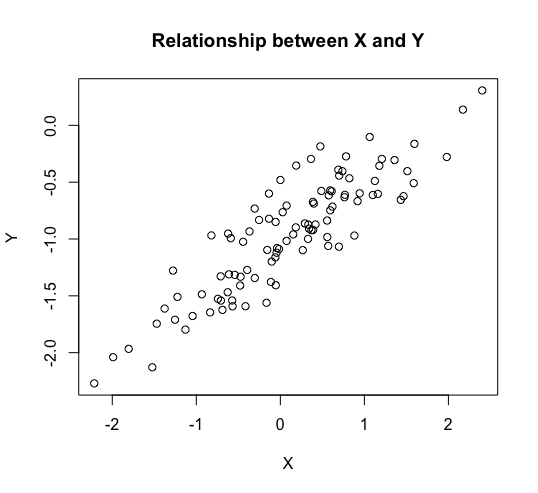
\includegraphics[width=0.45\textwidth]{HW1_P3_d.png}
\end{center}
\label{fig:HW1_P3_d}
\end{figure*}\\
\textbf{Ans:}\\
There is an approximate linear relationship between Y and X.

\subsection*{(e)}
\textbf{Code:}
\begin{lstlisting}[language=R]
> lm.fit = lm(y~x)
> summary(lm.fit)
> plot(x, y, xlab="X", ylab="Y", main="Relationship between X and Y")
> abline(lm.fit)
\end{lstlisting}
\textbf{Result:}
\begin{lstlisting}[language=R]
Call:
lm(formula = y ~ x)

Residuals:
     Min       1Q   Median       3Q      Max 
-0.46921 -0.15344 -0.03487  0.13485  0.58654 

Coefficients:
            Estimate Std. Error t value Pr(>|t|)    
(Intercept) -1.00942    0.02425  -41.63   <2e-16 ***
x            0.49973    0.02693   18.56   <2e-16 ***
---
Signif. codes:  0 ‘***’ 0.001 ‘**’ 0.01 ‘*’ 0.05 ‘.’ 0.1 ‘ ’ 1

Residual standard error: 0.2407 on 98 degrees of freedom
Multiple R-squared:  0.7784,	Adjusted R-squared:  0.7762 
F-statistic: 344.3 on 1 and 98 DF,  p-value: < 2.2e-16
\end{lstlisting}
\begin{figure}[!h]
\begin{center}
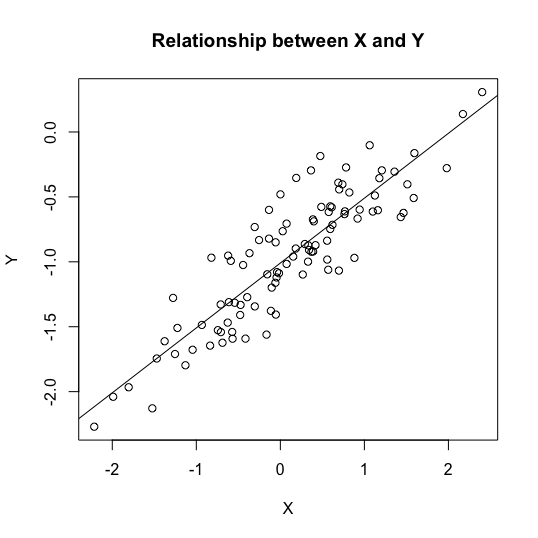
\includegraphics[width=0.5\textwidth]{HW1_P3_e.png}
\end{center}
\label{fig:HW1_P3_e}
\end{figure}
\textbf{Ans:}\\
$\hat{\beta}_0 = -1.00942$ \quad $\hat{\beta}_1 = 0.49973$ \qquad $\beta_0 = -1$ \quad $\beta_1 = 0.5$\\
With the $\mathrm{Pr}(>|t|) < 2e-16$, we will reject $H_0$ and say $\hat{\beta}_0$ and $\hat{\beta}_1$ are not 0.\\
With p-value $< 2.2e-16$ and $R^2 = 0.7784$, we can say there exist relationship between Y and X and our linear model fits Y and X well. \\
The estimated value of $\beta_0$ and $\beta_1$ are very close to their true value. 

\subsection*{(f)}
\textbf{Code:}
\begin{lstlisting}[language=R]
> par(col='black')
> plot(x, y, xlab="X", ylab="Y", main="Relationship between X and Y")
> abline(lm.fit, col='blue', lty=5)
> abline(a=-1, b=0.5, col='red', lty=1)
> legend('topleft', inset=0.05, c('least squares line', 'population regression line'), lty=c(5, 1), col=c('blue', 'red'), bty = "o")
\end{lstlisting}
\textbf{Result:}
\begin{figure}[!h]
\begin{center}
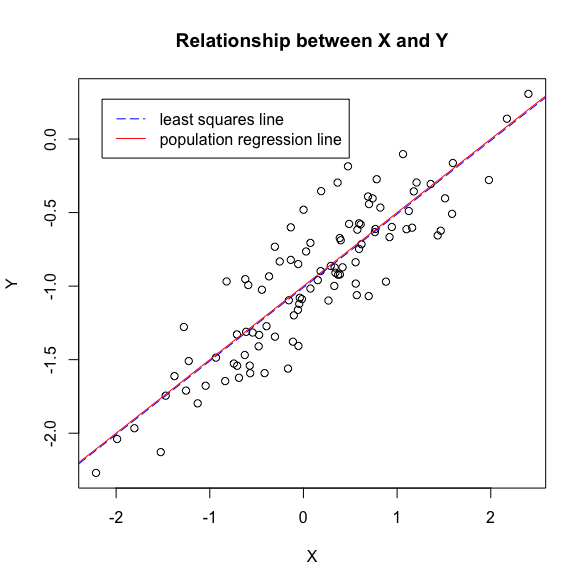
\includegraphics[width=0.7\textwidth]{HW1_P3_f.png}
\end{center}
\label{fig:HW1_P3_f}
\end{figure}

\subsection*{(g)}
\textbf{Code:}
\begin{lstlisting}[language=R]
# polynomial regression
Poly_fit = lm(y ~ poly(x,2))
# show regression result
summary(Poly_fit)
# creat points to draw fitting line
xlims = range(x)
x.grid = seq(from=xlims[1], to=xlims[2])
preds = predict(Poly_fit, newdata=list(x=x.grid), se=TRUE)
# use standard error to creat wrapper line
se.bands = cbind(preds$fit+2*preds$se.fit, preds$fit-2*preds$se.fit)
# draw 
plot(x, y, xlab="X", ylab="Y", main='Degree-2 Polynomial', col="black")
lines(x.grid, preds$fit, lwd=2, col="blue", lty=1)
matlines(x.grid, se.bands, lwd=1, col="red", lty=5)
legend('topleft', inset=0.05, c('polynomial regression line', 'SE wrapper line'), lwd=c(2, 1), lty=c(1, 5), col=c('blue', 'red'), bty = "o")
\end{lstlisting}
\textbf{Result:}
\begin{figure}[htb]
\begin{center}
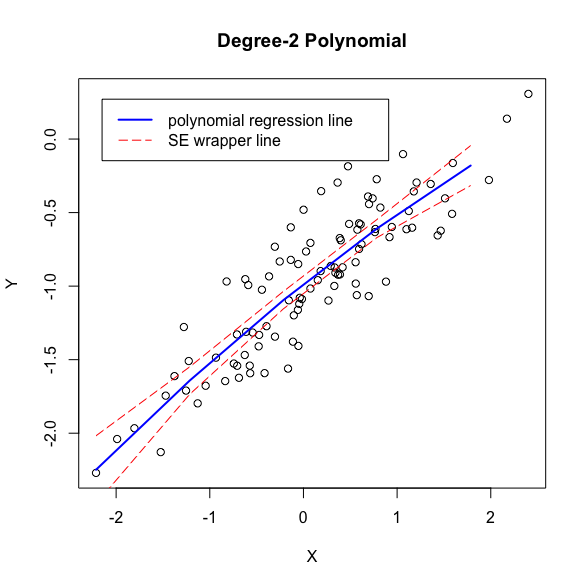
\includegraphics[width=0.7\textwidth]{HW1_P3_g.png}
\end{center}
\label{fig:HW1_P3_g}
\end{figure}
\begin{lstlisting}[language=R]
Call:
lm(formula = y ~ poly(x, 2))

Residuals:
    Min      1Q  Median      3Q     Max 
-0.4913 -0.1563 -0.0322  0.1451  0.5675 

Coefficients:
            Estimate Std. Error t value Pr(>|t|)    
(Intercept) -0.95501    0.02395 -39.874   <2e-16 ***
poly(x, 2)1  4.46612    0.23951  18.647   <2e-16 ***
poly(x, 2)2 -0.33602    0.23951  -1.403    0.164    
---
Signif. codes:  0 ‘***’ 0.001 ‘**’ 0.01 ‘*’ 0.05 ‘.’ 0.1 ‘ ’ 1

Residual standard error: 0.2395 on 97 degrees of freedom
Multiple R-squared:  0.7828,	Adjusted R-squared:  0.7784 
F-statistic: 174.8 on 2 and 97 DF,  p-value: < 2.2e-16
\end{lstlisting}
\textbf{Ans:}\\
There is limited evidence that the quadratic term improves the model fit. \\
The $\mathrm{Pr}(>|t|)$ of the quadratic term equals 0.164. So we still can say there's no relation between Y and $X^2$ with the probability equalling 0.164, which is not a small enough probability. \\
Also, from the figure above, the polynomial regression line is very close to the least squares line in linear model. \\
Therefore, the quadratic term hardly improves the model fit.

\subsection*{(h)}
\textbf{Code:}
\begin{lstlisting}[language=R]
# a
set.seed(1) # ensure consistent results
x=rnorm(100, mean=0, sd=1) # feature X

# b
eps=rnorm(100, mean=0, sd=0.1)

# c
y = -1 + 0.5*x + eps
length(y)

# d scatterplot
plot(x, y, xlab="X", ylab="Y", main="Relationship between X and Y")

# e least squares linear model
lm.fit = lm(y~x)
summary(lm.fit)
plot(x, y, xlab="X", ylab="Y", main="Relationship between X and Y")
abline(lm.fit)

# f 
par(col='black')
plot(x, y, xlab="X", ylab="Y", main="Relationship between X and Y")
abline(lm.fit, col='blue', lty=5) # least squares line
abline(a=-1, b=0.5, col='red', lty=1) # population regression line
legend('topleft', inset=0.05, c('least squares line', 'population regression line'), lty=c(5, 1), col=c('blue', 'red'), bty = "o")
\end{lstlisting}
\textbf{Result:}
\begin{figure}[htb]
\begin{center}
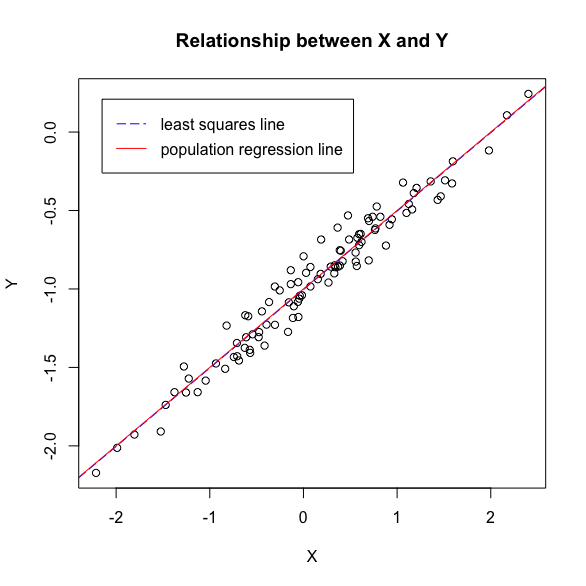
\includegraphics[width=0.7\textwidth]{HW1_P3_h.png}
\end{center}
\label{fig:HW1_P3_h}
\end{figure}
\begin{lstlisting}[language=R]
Call:
lm(formula = y ~ x)

Residuals:
     Min       1Q   Median       3Q      Max 
-0.18768 -0.06138 -0.01395  0.05394  0.23462 

Coefficients:
             Estimate Std. Error t value Pr(>|t|)    
(Intercept) -1.003769   0.009699  -103.5   <2e-16 ***
x            0.499894   0.010773    46.4   <2e-16 ***
---
Signif. codes:  0 ‘***’ 0.001 ‘**’ 0.01 ‘*’ 0.05 ‘.’ 0.1 ‘ ’ 1

Residual standard error: 0.09628 on 98 degrees of freedom
Multiple R-squared:  0.9565,	Adjusted R-squared:  0.956 
F-statistic:  2153 on 1 and 98 DF,  p-value: < 2.2e-16
\end{lstlisting}
\textbf{Ans:}\\
With less noise in the data, the observation points are more near to the population regression line. The estimated value of $\beta_0$ and $\beta_1$ are more close to their true value. $R^2 = 0.9565$ means the linear model gives a better fit. 

\subsection*{(i)}
\textbf{Code:}
\begin{lstlisting}[language=R]
# a
set.seed(1) # ensure consistent results
x=rnorm(100, mean=0, sd=1) # feature X

# b
eps=rnorm(100, mean=0, sd=1)

# c
y = -1 + 0.5*x + eps
length(y)

# d scatterplot
plot(x, y, xlab="X", ylab="Y", main="Relationship between X and Y")

# e least squares linear model
lm.fit = lm(y~x)
summary(lm.fit)
plot(x, y, xlab="X", ylab="Y", main="Relationship between X and Y")
abline(lm.fit)

# f 
par(col='black')
plot(x, y, xlab="X", ylab="Y", main="Relationship between X and Y")
abline(lm.fit, col='blue', lty=5) # least squares line
abline(a=-1, b=0.5, col='red', lty=1) # population regression line
legend('topleft', inset=0.05, c('least squares line', 'population regression line'), lty=c(5, 1), col=c('blue', 'red'), bty = "o")
\end{lstlisting}
\textbf{Result:}
\begin{lstlisting}[language=R]
Call:
lm(formula = y ~ x)

Residuals:
    Min      1Q  Median      3Q     Max 
-1.8768 -0.6138 -0.1395  0.5394  2.3462 

Coefficients:
            Estimate Std. Error t value Pr(>|t|)    
(Intercept) -1.03769    0.09699 -10.699  < 2e-16 ***
x            0.49894    0.10773   4.632 1.12e-05 ***
---
Signif. codes:  0 ‘***’ 0.001 ‘**’ 0.01 ‘*’ 0.05 ‘.’ 0.1 ‘ ’ 1

Residual standard error: 0.9628 on 98 degrees of freedom
Multiple R-squared:  0.1796,	Adjusted R-squared:  0.1712 
F-statistic: 21.45 on 1 and 98 DF,  p-value: 1.117e-05
\end{lstlisting}
\begin{figure}[htb]
\begin{center}
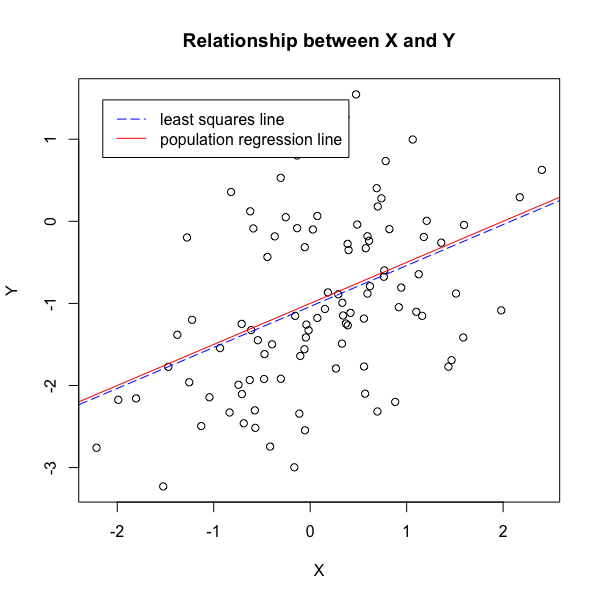
\includegraphics[width=0.7\textwidth]{HW1_P3_i.png}
\end{center}
\label{fig:HW1_P3_i}
\end{figure}
\textbf{Ans:}\\
With more noise in the data, the observation points are more far to the population regression line. The estimated value of $\beta_0$ and $\beta_1$ are more different to their true value. $R^2 = 0.1796$ means the linear model gives a worse fit. 

\subsection*{(j)}
\textbf{Code:}
\begin{lstlisting}[language=R]
confint(lm.fit)
\end{lstlisting}
\textbf{Result:}\\
$\epsilon \thicksim N(0, 0.25)$
\begin{lstlisting}[language=R]
                 2.5 %     97.5 %
(Intercept) -1.0575402 -0.9613061
x            0.4462897  0.5531801
\end{lstlisting}
$\epsilon \thicksim N(0, 0.1)$
\begin{lstlisting}[language=R]
                 2.5 %     97.5 %
(Intercept) -1.0230161 -0.9845224
x            0.4785159  0.5212720
\end{lstlisting}
$\epsilon \thicksim N(0, 1)$
\begin{lstlisting}[language=R]
                 2.5 %     97.5 %
(Intercept) -1.2301607 -0.8452245
x            0.2851588  0.7127204
\end{lstlisting}
\textbf{Ans:}\\
With less noise, the confidence interval for $\beta_0$ and $\beta_1$ are shorter, meaning the estimation are more accurate to the true value. \\
With more noise, the confidence interval for $\beta_0$ and $\beta_1$ are longer, meaning the estimation are less accurate to the true value. 

\newpage

\section*{P4}
\textbf{Code:}
\begin{lstlisting}[language=R]
Advertising = read.csv("/Users/yangchenye/Downloads/Advertising.csv",header=T,na.strings="?") 
dim(Advertising)
Advertising=na.omit(Advertising) # remove incomplete cases
dim(Advertising)
names(Advertising)
attach(Advertising)

# TV
TV_fit = lm(sales~TV) # least squares model
TV_CI = confint(TV_fit, level = 0.92) # 92% confidence intervals

plot(TV, sales, xlab="TV advertising", ylab="Sales", main="Relationship between Sales and TV advertising") # scatterplot
abline(TV_fit, col='blue', lty=1) # least squares line
abline(a=TV_CI[1,1], b=TV_CI[2,1], col='red', lty=5) # 92% confidence intervals line
abline(a=TV_CI[1,2], b=TV_CI[2,2], col='red', lty=5) # 92% confidence intervals line
legend('topleft', inset=0.05, c('least squares line', '92% confidence intervals line'), lty=c(1, 5), col=c('blue', 'red'), bty = "o")

# Radio
Radio_fit = lm(sales~radio) # least squares model
Radio_CI = confint(Radio_fit, level = 0.92) # 92% confidence intervals

plot(radio, sales, xlab="Radio advertising", ylab="Sales", main="Relationship between Sales and Radio advertising") # scatterplot
abline(Radio_fit, col='blue', lty=1) # least squares line
abline(a=Radio_CI[1,1], b=Radio_CI[2,1], col='red', lty=5) # 92% confidence intervals line
abline(a=Radio_CI[1,2], b=Radio_CI[2,2], col='red', lty=5) # 92% confidence intervals line
legend('topleft', inset=0.05, c('least squares line', '92% confidence intervals line'), lty=c(1, 5), col=c('blue', 'red'), bty = "o")

# Newspaper
Newspaper_fit = lm(sales~newspaper) # least squares model
Newspaper_CI = confint(Newspaper_fit, level = 0.92) # 92% confidence intervals

plot(newspaper, sales, xlab="Newspaper advertising", ylab="Sales", main="Relationship between Sales and Newspaper advertising") # scatterplot
abline(Newspaper_fit, col='blue', lty=1) # least squares line
abline(a=Newspaper_CI[1,1], b=Newspaper_CI[2,1], col='red', lty=5) # 92% confidence intervals line
abline(a=Newspaper_CI[1,2], b=Newspaper_CI[2,2], col='red', lty=5) # 92% confidence intervals line
legend('bottomright', inset=0.05, c('least squares line', '92% confidence intervals line'), lty=c(1, 5), col=c('blue', 'red'), bty = "o")
\end{lstlisting}
\textbf{Result:}
\begin{lstlisting}[language=R]
> TV_CI
                   4 %       96 %
(Intercept) 6.22691926 7.83826784
TV          0.04280193 0.05227135
> Radio_CI
                  4 %       96 %
(Intercept) 8.3210922 10.3021840
radio       0.1665776  0.2384139
> Newspaper_CI
                    4 %        96 %
(Intercept) 11.25788302 13.44493112
newspaper    0.02552451  0.08386169
\end{lstlisting}
\begin{figure}[!h]
\begin{center}
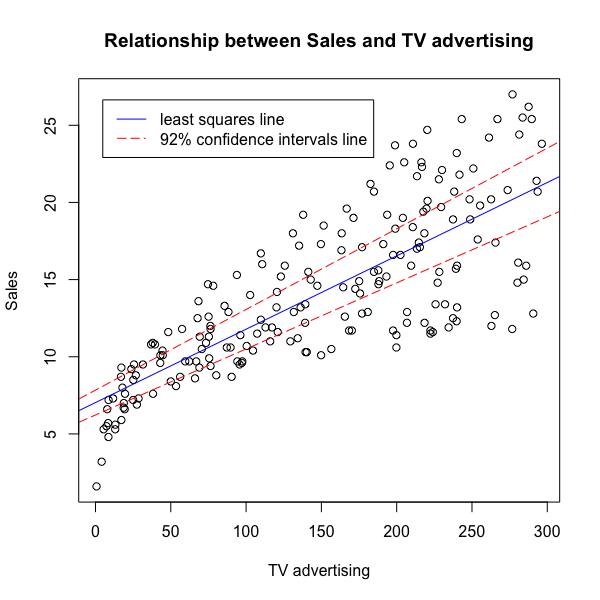
\includegraphics[width=0.6\textwidth]{HW1_P4_1.png}
\end{center}
\newpage
\label{fig:HW1_P4_1}
\end{figure}
\begin{figure}[!h]
\begin{center}
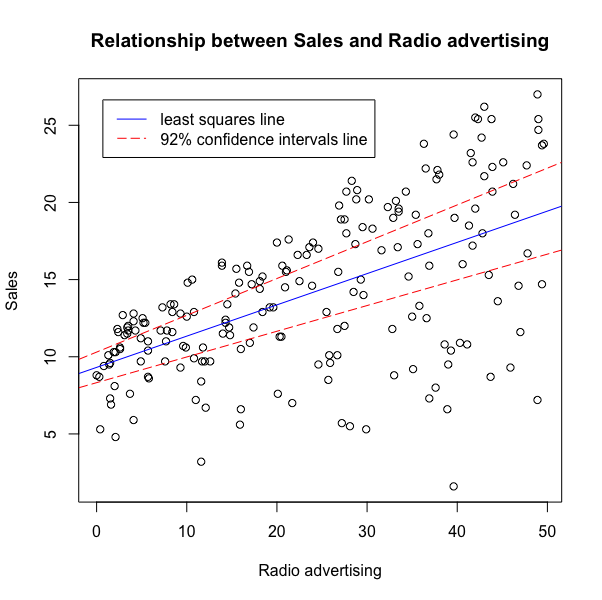
\includegraphics[width=0.6\textwidth]{HW1_P4_2.png}
\end{center}
\label{fig:HW1_P4_2}
\end{figure}
\newpage
\begin{figure}[!h]
\begin{center}
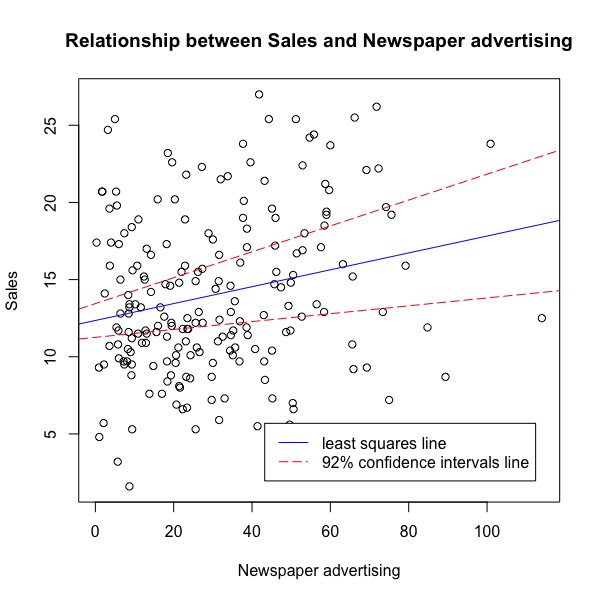
\includegraphics[width=0.6\textwidth]{HW1_P4_3.png}
\end{center}
\label{fig:HW1_P4_3}
\end{figure}


\newpage

\section*{P5}
\subsection*{(a)}
\textbf{Code:}
\begin{lstlisting}[language=R]
Auto = read.csv("/Users/yangchenye/Downloads/Auto.csv",header=T,na.strings="?") 
dim(Auto)
Auto=na.omit(Auto) # remove incomplete cases
dim(Auto)
names(Auto)
attach(Auto)
pairs(Auto)
\end{lstlisting}
\textbf{Result:}
\begin{figure}[!h]
\begin{center}
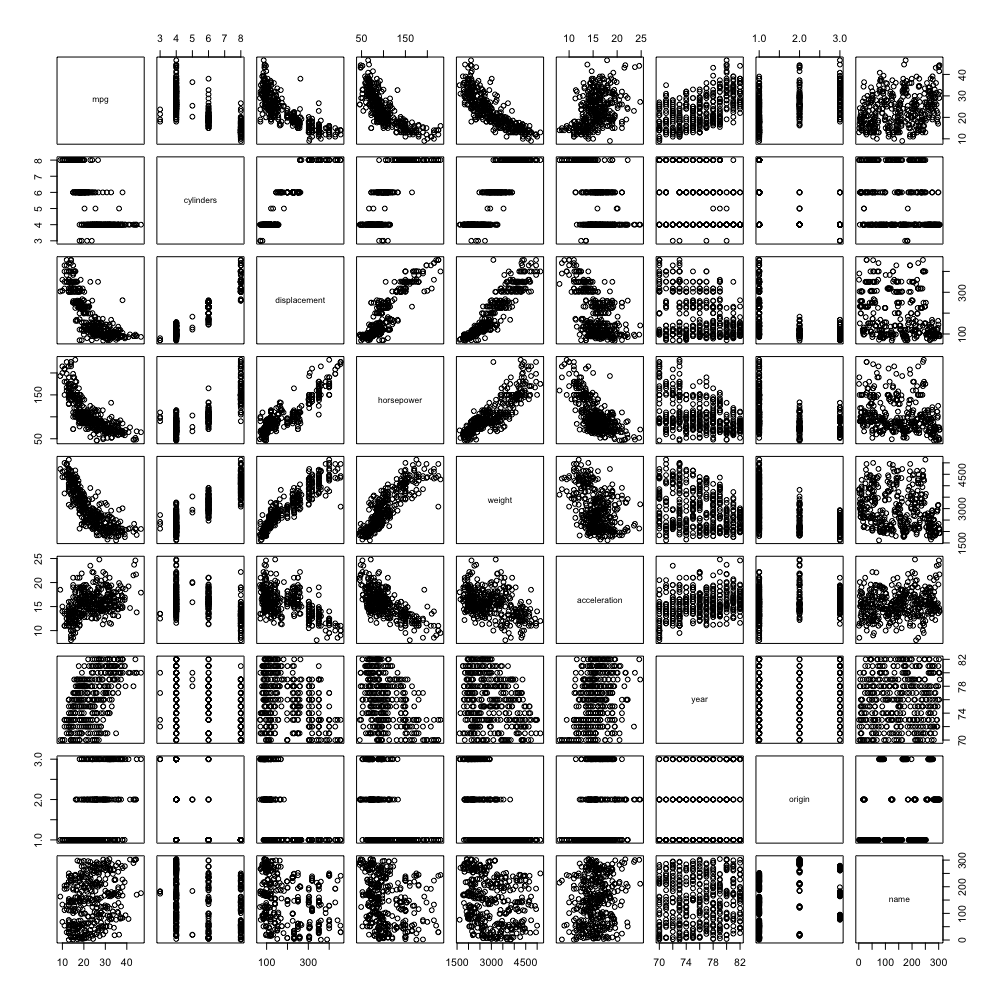
\includegraphics[width=0.88\textwidth]{HW1_P5_a.png}
\end{center}
\label{fig:HW1_P5_a}
\end{figure}


\subsection*{(b)}
\textbf{Code:}
\begin{lstlisting}[language=R]
CRM = cor(Auto[,1:8])
\end{lstlisting}
\textbf{Result:}
\begin{lstlisting}[language=R, basicstyle=\tiny]
                    mpg  cylinders displacement horsepower     weight acceleration       year     origin
mpg           1.0000000 -0.7776175   -0.8051269 -0.7784268 -0.8322442    0.4233285  0.5805410  0.5652088
cylinders    -0.7776175  1.0000000    0.9508233  0.8429834  0.8975273   -0.5046834 -0.3456474 -0.5689316
displacement -0.8051269  0.9508233    1.0000000  0.8972570  0.9329944   -0.5438005 -0.3698552 -0.6145351
horsepower   -0.7784268  0.8429834    0.8972570  1.0000000  0.8645377   -0.6891955 -0.4163615 -0.4551715
weight       -0.8322442  0.8975273    0.9329944  0.8645377  1.0000000   -0.4168392 -0.3091199 -0.5850054
acceleration  0.4233285 -0.5046834   -0.5438005 -0.6891955 -0.4168392    1.0000000  0.2903161  0.2127458
year          0.5805410 -0.3456474   -0.3698552 -0.4163615 -0.3091199    0.2903161  1.0000000  0.1815277
origin        0.5652088 -0.5689316   -0.6145351 -0.4551715 -0.5850054    0.2127458  0.1815277  1.0000000
\end{lstlisting}


\subsection*{(c)}
\textbf{Code:}
\begin{lstlisting}[language=R]
mlm_fit = lm(mpg~cylinders + displacement + horsepower + weight + acceleration + year + origin)
summary(mlm_fit)
\end{lstlisting}
\textbf{Result:}
\begin{lstlisting}[language=R]
Call:
lm(formula = mpg ~ cylinders + displacement + horsepower + weight + 
    acceleration + year + origin)

Residuals:
    Min      1Q  Median      3Q     Max 
-9.5903 -2.1565 -0.1169  1.8690 13.0604 

Coefficients:
               Estimate Std. Error t value Pr(>|t|)    
(Intercept)  -17.218435   4.644294  -3.707  0.00024 ***
cylinders     -0.493376   0.323282  -1.526  0.12780    
displacement   0.019896   0.007515   2.647  0.00844 ** 
horsepower    -0.016951   0.013787  -1.230  0.21963    
weight        -0.006474   0.000652  -9.929  < 2e-16 ***
acceleration   0.080576   0.098845   0.815  0.41548    
year           0.750773   0.050973  14.729  < 2e-16 ***
origin         1.426141   0.278136   5.127 4.67e-07 ***
---
Signif. codes:  0 ‘***’ 0.001 ‘**’ 0.01 ‘*’ 0.05 ‘.’ 0.1 ‘ ’ 1

Residual standard error: 3.328 on 384 degrees of freedom
Multiple R-squared:  0.8215,	Adjusted R-squared:  0.8182 
F-statistic: 252.4 on 7 and 384 DF,  p-value: < 2.2e-16
\end{lstlisting}
\textbf{Ans:}\\
\textbf{i. Is there a relationship between the predictors and the response?}\\
With the p-value $< 2.2e-16$, we should reject $H_0$, namely, admit that there exist a relationship between predictors and response. And $R^2=0.8215$ shows that this linear model fits the data well. \\
\textbf{ii. Which predictors appear to have a statistically significant relationship to the response?}\\
The $\mathrm{Pr}(>|t|)$ of cylinders, horsepower and acceleration are not small enough to say they have significant relationship to the response, while the $\mathrm{Pr}(>|t|)$ of other predictors are small enough. That is to say, displacement, weight, year and origin have a statistically significant relationship to the response mpg. \\
\textbf{iii. What does the coefficient for the year variable suggest?}\\
The estimated coefficient for the year variable is 0.750773, suggesting that with one unit increase in year, the mpg will increases about 0.75 unit. The year has a positive relationship to mpg. 

\subsection*{(d)}
\textbf{Code:}
\begin{lstlisting}[language=R]
mlm_fit_log = lm(log10(mpg)~log10(cylinders) + log10(displacement) +log10(horsepower) + log10(weight) + log10(acceleration) + log10(year) + log10(origin))
summary(mlm_fit_log)

mlm_fit_sqrt = lm(sqrt(mpg)~sqrt(cylinders) + sqrt(displacement) +sqrt(horsepower) + sqrt(weight) + sqrt(acceleration) + sqrt(year) + sqrt(origin))
summary(mlm_fit_sqrt)

mlm_fit_power = lm(mpg^2~cylinders^2 + displacement^2 + horsepower^2 + weight^2 + acceleration^2 + year^2 + origin^2)
summary(mlm_fit_power)
\end{lstlisting}
\textbf{Result with the transformation of $\mathrm{log}(x)$:}
\begin{lstlisting}[language=R]
Call:
lm(formula = log10(mpg) ~ log10(cylinders) + log10(displacement) + 
    log10(horsepower) + log10(weight) + log10(acceleration) + 
    log10(year) + log10(origin))

Residuals:
      Min        1Q    Median        3Q       Max 
-0.179356 -0.030825  0.000238  0.026708  0.171685 

Coefficients:
                     Estimate Std. Error t value Pr(>|t|)    
(Intercept)         -0.067485   0.281523  -0.240  0.81068    
log10(cylinders)    -0.082815   0.061429  -1.348  0.17841    
log10(displacement)  0.006625   0.056970   0.116  0.90748    
log10(horsepower)   -0.294389   0.057652  -5.106 5.18e-07 ***
log10(weight)       -0.569666   0.082397  -6.914 1.98e-11 ***
log10(acceleration) -0.179239   0.059536  -3.011  0.00278 ** 
log10(year)          2.243989   0.131661  17.044  < 2e-16 ***
log10(origin)        0.044848   0.018821   2.383  0.01767 *  
---
Signif. codes:  0 ‘***’ 0.001 ‘**’ 0.01 ‘*’ 0.05 ‘.’ 0.1 ‘ ’ 1

Residual standard error: 0.04935 on 384 degrees of freedom
Multiple R-squared:  0.8903,	Adjusted R-squared:  0.8883 
F-statistic: 445.3 on 7 and 384 DF,  p-value: < 2.2e-16
\end{lstlisting}
\textbf{Result with the transformation of $\sqrt{x}$:}
\begin{lstlisting}[language=R]
Call:
lm(formula = sqrt(mpg) ~ sqrt(cylinders) + sqrt(displacement) + 
    sqrt(horsepower) + sqrt(weight) + sqrt(acceleration) + sqrt(year) + 
    sqrt(origin))

Residuals:
     Min       1Q   Median       3Q      Max 
-0.98667 -0.17280 -0.00315  0.16145  1.02245 

Coefficients:
                    Estimate Std. Error t value Pr(>|t|)    
(Intercept)        -1.949286   0.847481  -2.300 0.021979 *  
sqrt(cylinders)    -0.108552   0.141968  -0.765 0.444964    
sqrt(displacement)  0.019707   0.021182   0.930 0.352752    
sqrt(horsepower)   -0.090896   0.028428  -3.197 0.001502 ** 
sqrt(weight)       -0.061414   0.007292  -8.422 7.48e-16 ***
sqrt(acceleration) -0.107258   0.077048  -1.392 0.164699    
sqrt(year)          1.266015   0.079308  15.963  < 2e-16 ***
sqrt(origin)        0.272324   0.070883   3.842 0.000143 ***
---
Signif. codes:  0 ‘***’ 0.001 ‘**’ 0.01 ‘*’ 0.05 ‘.’ 0.1 ‘ ’ 1

Residual standard error: 0.2964 on 384 degrees of freedom
Multiple R-squared:  0.8662,	Adjusted R-squared:  0.8638 
F-statistic: 355.1 on 7 and 384 DF,  p-value: < 2.2e-16
\end{lstlisting}
\textbf{Result with the transformation of $x^2$:}
\begin{lstlisting}[language=R]
Call:
lm(formula = mpg^2 ~ cylinders^2 + displacement^2 + horsepower^2 + 
    weight^2 + acceleration^2 + year^2 + origin^2)

Residuals:
    Min      1Q  Median      3Q     Max 
-483.45 -141.87  -19.62  103.58 1042.84 

Coefficients:
               Estimate Std. Error t value Pr(>|t|)    
(Intercept)  -1.878e+03  2.928e+02  -6.412 4.22e-10 ***
cylinders    -1.436e+01  2.038e+01  -0.704  0.48157    
displacement  1.328e+00  4.738e-01   2.802  0.00534 ** 
horsepower   -3.587e-01  8.693e-01  -0.413  0.68009    
weight       -3.522e-01  4.111e-02  -8.567 2.62e-16 ***
acceleration  9.278e+00  6.232e+00   1.489  0.13740    
year          4.081e+01  3.214e+00  12.698  < 2e-16 ***
origin        9.509e+01  1.754e+01   5.422 1.04e-07 ***
---
Signif. codes:  0 ‘***’ 0.001 ‘**’ 0.01 ‘*’ 0.05 ‘.’ 0.1 ‘ ’ 1

Residual standard error: 209.8 on 384 degrees of freedom
Multiple R-squared:  0.7292,	Adjusted R-squared:  0.7243 
F-statistic: 147.8 on 7 and 384 DF,  p-value: < 2.2e-16
\end{lstlisting}
\textbf{Ans:}\\
Different transformations of variables will lead to different estimate value of parameters in a same linear model. For example, the intercepts corresponding with different transformation are −17.218435, −0.067485, −1.949286 and −1.878e+03. \\
Also, transformations will change the relationship between variables. For example, "displacement" has relationship with "mpg" in $x$ and $x^2$ transformation situation, while little relationship in $\mathrm{log}(x)$ and $\sqrt{x}$ situation.\\
Moreover, transformation on variables will also change the property of the linear model, which can be seen in the difference of $R^2$, RSE and F - statistic. 


\newpage

\section*{P6}
\textbf{Ans:}\\
From the given constrain, we can calculate the following values:\\
\begin{equation}
    \begin{aligned}
    &\bar{x} = \frac{1}{n} \sum_{i=1}^{n} x_i = \frac{1}{20} \sum_{i=1}^{20} x_i = \frac{1}{20} \times 8.552 = 0.4276\\
    &\bar{y} = \frac{1}{n} \sum_{i=1}^{n} y_i = \frac{1}{20} \sum_{i=1}^{20} y_i = \frac{1}{20} \times 398.2 = 19.91\\
    \end{aligned}
\end{equation}{}
\begin{equation}
    \begin{aligned}
    \sum_{i=1}^n (x_i - \bar{x}) (y_i - \bar{y}) &= \sum_{i=1}^{20} (x_i y_i - \bar{x} y_i - x_i \bar{y} + \bar{x}\bar{y})\\
    &= \sum_{i=1}^{20} (x_i y_i) - \bar{x} \sum_{i=1}^{20} y_i - \bar{y} \sum_{i=1}^{20} x_i + 20\bar{x}\bar{y}\\
    &= 216.6 - 0.4276\times 398.2 - 19.91\times 8.552 + 20 \times 0.4276 \times 19.91\\
    &= 46.33\\
    \sum_{i=1}^n (x_i - \bar{x})^2 &= \sum_{i=1}^{20} (x_i^2 - 2\bar{x} x_i  + \bar{x}^2)\\
    &= \sum_{i=1}^{20} x_i^2 - 2\bar{x} \sum_{i=1}^{20} x_i  + 20\bar{x}^2\\
    &= 5.196 - 2\times0.4276\times8.552 + 20\times0.4276^2\\
    &= 1.539\\
    \sum_{i=1}^n (y_i - \bar{y})^2 &= \sum_{i=1}^{20} (y_i^2 - 2\bar{y} y_i  + \bar{y}^2)\\
    &= \sum_{i=1}^{20} y_i^2 - 2\bar{y} \sum_{i=1}^{20} y_i  + 20\bar{y}^2\\
    &= 9356 - 2\times19.91\times398.2 + 20\times19.91^2\\
    &= 1428
    \end{aligned}
\end{equation}{}\\
Thus:\\
\begin{equation}
    \begin{aligned}
    \hat{\beta}_1 &= \frac{\sum_{i=1}^n (x_i-\bar{x})(y_i-\bar{y})}{\sum_{i=1}^n (x_i-\bar{x})^2} = \frac{46.33}{1.539} = 30.10\\
    \hat{\beta}_0 &= \bar{y} - \hat{\beta}_1\bar{x} = 19.91 - 30.10\times 0.4276 = 7.039\\
    \mathrm{RSS} &= \sum_{i=1}^n (y_i-\hat{y}_i)^2 = \sum_{i=1}^n (y_i - \hat{\beta}_0 - \hat{\beta}_1 x_i)^2 = \sum_{i=1}^n (y_i - \bar{y} + \hat{\beta}_1 \bar{x} - \hat{\beta}_1 x_i)^2 \\
    &= \sum_{i=1}^n (y_i - \bar{y})^2 - \hat{\beta}_1 \sum_{i=1}^n (y_i - \bar{y}) (x_i - \bar{x}) = 1428 - 30.10\times 46.33 = 33.47
    \end{aligned}
\end{equation}{}\\
\begin{equation}
\begin{aligned}
R^2 &= 1 - \frac{\mathrm{RSS}}{\sum_{i=1}^n (y_i-\bar{y})^2} = 1-\frac{33.47}{1428} = 0.9766\\
\hat{\sigma}^2 &= \frac{\mathrm{RSS}}{n-2}  = \frac{\mathrm{33.47}}{20-2} = 1.859
\end{aligned}
\end{equation}{}\\

When $x = 0.5$:\\
$$\hat{y} = \hat{\beta}_0 + \hat{\beta}_1 x = 7.039 + 30.10\times 0.5 = 22.09$$\\



\newpage

\section*{P7}
\textbf{Code:}
\begin{lstlisting}[language=Matlab]
fcdf(1.89, 6, 38, 'upper') % matlab
\end{lstlisting}{}
\textbf{Ans:}\\
The null hypothesis test is performed by computing the F-statistic:\\
\begin{equation}
\begin{aligned}
&F = \frac{(\mathrm{TSS}-\mathrm{RSS})/p}{\mathrm{RSS}/(n-p-1)} = \frac{(11.62-8.95)/6}{8.95/(45-6-1)} = 1.89\\
&\mathrm{Pr} (F_{6,38} > 1.89) = 0.11
\end{aligned}
\end{equation}{}\\
The $p$-value for the null hypothesis is 0.11


\newpage

\section*{E1}
\textbf{Ans:}\\
The definition of gamma function is :
$$\Gamma(x) = \int_{0}^{+\infty} t^{x-1} e^{-t} dt $$
If a random variable $X \thicksim \Gamma(\alpha, \theta) $, then the probability density function of $X$ has the following format:\\
\begin{equation}
    \centering
    f_X (x)=
    \left\{  
             \begin{aligned}
             \frac{1}{\theta^\alpha \Gamma(\alpha)}x^{\alpha-1}e^{-x/\theta}&, x > 0 \\
             0\qquad\qquad&, \mathrm{else}
             \end{aligned}
    \right. 
\end{equation}{}\\
Let the density of $X$ be $f_X (x)$, and let the density of $Y=X^2$ be $f_Y (y)$, we have:\\
\begin{equation}
    \centering
    f_Y (y)=
    \left\{  
             \begin{aligned}
             \frac{1}{2\sqrt{y}}[f_X(\sqrt{y}) + f_X(-\sqrt{y})]&, y > 0 \\
             0\qquad\qquad\qquad&, \mathrm{else}
             \end{aligned}
    \right. 
\end{equation}{}\\
Therefore, as for random variable $X \thicksim N(0,1)$ with density $\varphi (x)=\frac{1}{\sqrt{2\pi}}e^{-x^2/2}\ (-\infty<x<\infty)$, let $Y=X^2$, the density of $Y$ is:
\begin{equation}
    \centering
    \begin{aligned}
    f_Y (y)&=
    \left\{  
             \begin{aligned}
             \frac{1}{2\sqrt{y}}[\frac{1}{\sqrt{2\pi}}e^{-y/2} + \frac{1}{\sqrt{2\pi}}e^{-y/2}]&, y > 0 \\
             0\qquad\qquad\qquad&, \mathrm{else}
             \end{aligned}
    \right. \\
    &=
    \left\{  
             \begin{aligned}
             \frac{1}{\sqrt{2\pi}}\frac{1}{\sqrt{y}} e^{-y/2}&, y > 0 \\
             0\qquad&, \mathrm{else}
             \end{aligned}
    \right. \\
    \end{aligned}
\end{equation}{}\\
Thus, $Y=X^2 \thicksim \Gamma(\frac{1}{2}, 2)$.\\
Because $X_i,\ i=1,...,n$ are independent, and as a result $X_i^2,\ i=1,...,n$ are also independent, Chi-squared distribution $\chi_n^2 = X_1^2 + X_2^2 + ... + X_n^2$ has additivity. Namely:\\
$$\chi_n^2 = \sum_{i=1}^{n} X_i^2 \thicksim \Gamma(\frac{n}{2}, 2)$$
Therefore, the density of $\chi_n^2$ is given by:
\begin{equation}
    \centering
    g_n (x)=
    \left\{  
             \begin{aligned}
             \frac{1}{2^{n/2}\Gamma(n/2)} x^{n/2-1} e^{-x/2}&, x > 0 \\
             0\qquad\qquad\qquad&, x \leq 0
             \end{aligned}
    \right. 
\end{equation}{}\\

\newpage

\section*{E2}
\textbf{Ans:}\\
(The first half of the proof is the same as P1(d), I just copy and paste.)\\
Let $Z_i = \frac{X_i -\mu}{\sigma}\ i=1,2,...,n$, thus $Z_1, Z_2,..., Z_n$ are independent and $Z_i\thicksim N(0,1)\ i=1,2,...,n$. Also:\\
\begin{equation}
    \begin{aligned}
    \bar{Z} &= \frac{1}{n}\sum_{i=1}^{n} Z_i = \frac{1}{n}\sum_{i=1}^{n} \frac{X_i -\mu}{\sigma} = \frac{\bar{X}-\mu}{\sigma}\\
    \frac{(n-1)S^2}{\sigma^2} &= \frac{\sum_{i=1}^{n} (X_i - \bar{X})^2}{\sigma^2} = \sum_{i=1}^{n} [\frac{ (X_i - \mu) - (\bar{X} - \mu)}{\sigma }]^2\\
    &= \sum_{i=1}^{n} (Z_i - \bar{Z})^2 = \sum_{i=1}^{n} (Z_i^2 - 2Z_i\bar{Z} + \bar{Z}^2)\\
    &= \sum_{i=1}^{n}Z_i^2 - 2\bar{Z}\sum_{i=1}^{n}Z_i + n\bar{Z}^2 = \sum_{i=1}^{n}Z_i^2 - n\bar{Z}^2
    \end{aligned}
\end{equation}
Choose a matrix $\bm{A} = (a_{ij})$, in which all the entries in the first row are $1/\sqrt{n}$, and each row vector of the matrix should be orthogonal. Do:\\
$$\bm{Y} = \bm{AZ}$$
In which $$\bm{Y} = (Y_1, Y_2,...,Y_n)^T$$ $$\bm{Z} = (Z_1, Z_2,...,Z_n)^T$$ $$\bm{A} = (\bm{a_1}^T, \bm{a_2}^T,...,\bm{a_n}^T)^T$$
Because $Y_i$ is the linear combination of $Z_i$ and $Z_i\thicksim N(0,1)\ i=1,2,...,n$, therefore $Y_i\ i=1,2,...,n$ have normal/Gaussian distribution and:
\begin{equation}
\begin{aligned}
\mathbb{E}(Y_i) &= \mathbb{E}(\sum_{j=1}^{n} a_{ij}Z_j) = \sum_{j=1}^{n} a_{ij}\mathbb{E}(Z_j) = 0\\
\mathrm{Var}(Y_i) &= \mathrm{Var}(\sum_{j=1}^{n} a_{ij}Z_j) = \sum_{j=1}^{n} a_{ij}^2 = <\bm{a_i}, \bm{a_i}> = 1
\end{aligned}
\end{equation}\\
Because $\mathrm{Cov}(Z_k, Z_h)$ equals 1 when $k=h$ and equals 0 when $k\neq h$:
\begin{equation}
    \begin{aligned}
    \mathrm{Cov}(Y_i, Y_j) &= \mathrm{Cov}(\sum_{k=1}^{n} a_{ik}Z_k, \sum_{h=1}^{n} a_{jh}Z_h) \\
    &= \sum_{k=1}^{n} \sum_{h=1}^{n} a_{ik} a_{jh} \mathrm{Cov}(Z_k, Z_h) \\
    &= \sum_{k=1}^{n} a_{ik} a_{jk}\\
    &= <\bm{a_i}, \bm{a_j}>\\
    &=
    \left\{  
             \begin{aligned}
             1\qquad&, i=j \\
             0\qquad&, i\neq j
             \end{aligned}
    \right. \\
    &= \mathrm{Cov}(Z_i, Z_j)
    \end{aligned}
\end{equation}\\
Therefore, $Y_i\ i=1,2,...,n$ has no correlation with each other. Considering $Y_i \thicksim N(0,1)$, thus $Y_1, Y_2,..., Y_n$ are independent. 
Also:\\
\begin{equation}
\begin{aligned}
&Y_1 = \sum_{j=1}^{n} a_{1j}Z_j = \sum_{j=1}^{n}\frac{1}{\sqrt{n}}Z_j = \sqrt{n}\bar{Z}\\
&\sum_{i=1}^{n}Y_i^2 = \bm{Y}^T\bm{Y} = (\bm{AZ})^T(\bm{AZ}) = \bm{Z}^T (\bm{A} \bm{A}^T)^T \bm{Z} = \bm{Z}^T \bm{I} \bm{Z} = \sum_{i=1}^{n}Z_i^2
\end{aligned}
\end{equation}\\
Therefore:
\begin{equation}
\begin{aligned}
\frac{(n-1)S^2}{\sigma^2} = \sum_{i=1}^{n}Z_i^2 - n\bar{Z}^2 = \sum_{i=1}^{n}(Y_i^2) - Y_1^2 = \sum_{i=2}^{n}(Y_i^2)
\end{aligned}
\end{equation}\\
Because $Y_2, Y_3,..., Y_n$ are independent and $Y_i \thicksim N(0,1)\ i=2,3,...,n$, thus $\sum_{i=2}^{n}(Y_i^2)\thicksim \chi_{n-1}^2$. \\
Thus:
$$\frac{(n-1)S^2}{\sigma^2}\thicksim \chi_{n-1}^2$$
Namely:
$$\frac{(n-1)S^2}{\sigma^2}\overset{d}{=} \chi_{n-1}^2$$


\newpage

\section*{E3}
\textbf{Ans:}\\


\newpage

\section*{E4}
\textbf{Ans:}\\


\newpage

\end{document}